\section{METHODOLOGY}\label{SC:METHOD}\label{sec:methods}
SAD combines predictor preprocessing, anomaly screening, supervised
classification and batch-wise model updating. The following subsections
specify these components, their integration and the evaluation measures.

\subsection{PRE PROCESSING}\label{SSC:PreProcessing}
Dimensionality reduction decreases the number of input variables while
retaining useful characteristics of the data. In this research, the
preprocessing step uses feature screening through a Gini criterion for
categorical variables and a near-zero-variance criterion for numerical
variables \citep{Hastie2009,Kuhn2008}.

\subsubsection*{Dimension Reduction}
\textbf{Gini Index:} For a categorical predictor with category frequencies
$p_r$, the Gini impurity is
\[
Gini=1-\sum_{r=1}^{R}p_r^2.
\]
It is zero for a constant feature and increases as the observations are
distributed more evenly across categories. We retain predictors with
$g_L<Gini<g_U$, where $g_L=0.1$ and $g_U=0.9$.
\rev{This marginal variability screen does not measure association with fraud;
it can discard informative high-cardinality features.}

\textbf{Near Zero Variance:} Numerical predictors are removed if constant,
or if their most-common to second-most-common value frequency ratio exceeds
19 and their percentage of unique values is at most 10\%, following the
near-zero-variance screening convention \citep{Kuhn2008}.

\rev{To prevent information from later evaluation batches entering fitted
preprocessing, partitioning precedes feature screening. The screen, missing
value handling, scaling and categorical encoding are fitted using $D_1$
predictors only, as made explicit in Algorithm \ref{algo:preprocessing}.}
\begin{algorithm}[htbp]
\footnotesize
\caption{PreProcessing Algorithm}\label{algo:preprocessing}
\begin{algorithmic}[1]
\REQUIRE Dataset $D$; partition fractions $p_1,\ldots,p_m$; Gini bounds $g_L,g_U$
\ENSURE Partitions $D_1,\ldots,D_m$ and fixed predictor transformations
\STATE \rev{Withhold outcomes from predictors; retain original row identities.}
\STATE \rev{Partition records with sizes proportional to $p_1,\ldots,p_m$.}
\STATE \rev{On $D_1$ only, remove categorical predictors outside $(g_L,g_U)$ in Gini impurity.}
\STATE \rev{On $D_1$ only, remove numerical predictors satisfying near-zero variance.}
\STATE \rev{Fit imputation, scaling and encoding on retained $D_1$ predictors.}
\STATE \rev{Apply those fixed transformations to every partition $D_j$.}
\end{algorithmic}
\end{algorithm}


\begin{revised}
Policy identifiers, postal identifiers and incident addresses are excluded.
Near-unique categorical fields are also excluded. The two date fields in
Insurance Claims are expanded into year, month and weekday; this does not
make the experimental split chronological. The marker \texttt{?} is treated
as missing. Numerical medians and categorical modes provide imputation;
scaling and one-hot encoding use $D_1$ parameters and levels, with unseen
categories mapped to zero indicators. Outcomes are removed by name before
any detector or transformation is fitted, and row identities are preserved.
\end{revised}

\subsubsection*{Balancing}
\textbf{Resampling structure:} We use the Synthetic Minority Over-sampling
Technique (SMOTE) to address class imbalance during supervised training
\citep{Chawla2002,He2009}. SMOTE constructs additional minority-class
training vectors along line segments joining a minority observation to a
nearby observation from the same class.
\rev{In the revised experiments, SMOTE is applied only to accumulated
verified training records, never to future evaluation observations.
The neighbor count is at most five and is reduced for small minority sets.
One minority observation invokes random oversampling; a single-class set
raises an error. SMOTE operates on encoded features, so synthetic one-hot
values may be fractional. These are training vectors, not synthetic policies.
Previously generated synthetic records are not accumulated across rounds.}

\subsection*{Structure}
The two SAD workflows are illustrated below.
Figure \ref{figai1} connects preprocessing and data partitioning to
initial anomaly screening, verification and supervised learning. In subsequent iterations, the trained
models identify potential fraud in the next subset, followed by expert
confirmation and model updating.
Figure \ref{figai2} shows the multilayered structure, where EAD is applied
to the result of anomaly consensus before expert verification.
\rev{Figures 1 and 2 provide conceptual overviews of the retained workflows.
Algorithms 1--3 specify their implementation: preprocessing is fitted on $D_1$ after partitioning; expert review
includes alerts and a random sample of non-alerts; both fraud and genuine
verified records enter training (the diagram label ``Frauds'' is shorthand
for the reviewed records); and no model is retrained after the last evaluation
batch. The terminal trained model in the conceptual diagrams is relevant only
if further batches will arrive. Simple-A uses nine initial detector votes;
Simple-B adds entropy as a tenth vote. In Multilayer, EAD gates the initial
candidate subset before verification.}

\begin{figure}[!htbp]\centering
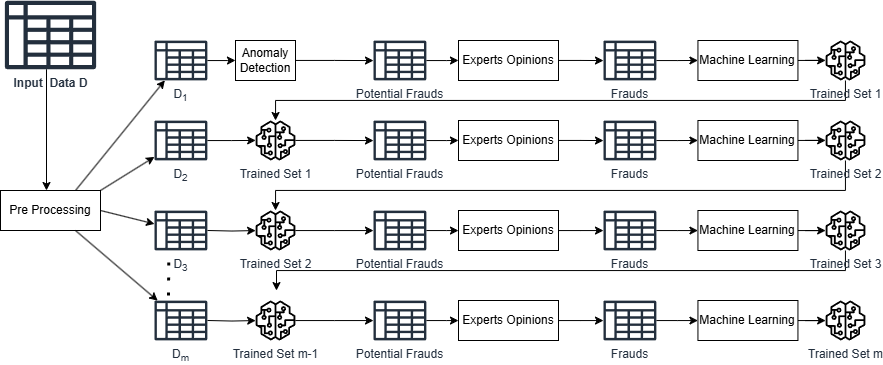
\includegraphics[width=\textwidth]{figures/simple.png}
\caption{Simple SAD workflow: initial screening, verification and model updating
across successive batches.}\label{figai1}
\medskip
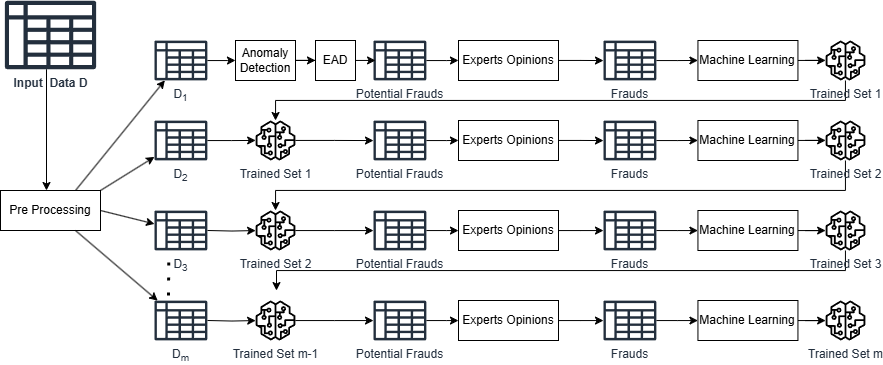
\includegraphics[width=\textwidth]{figures/Multilayered.png}
\caption{Multilayered SAD workflow, with entropy screening between initial
anomaly consensus and verification.}\label{figai2}
\end{figure}

\subsection*{ANOMALY DETECTION}\label{SSC:AD}
Before verified labels become available, the initial ensemble screens
claims for departures from empirical feature patterns. An anomaly flag
indicates a case for review, not a confirmed fraud \citep{Chandola2009}.
The nine retained detectors are specified below.

\textbf{Box Plot:} Observations outside
$[Q_1-1.5IQR,Q_3+1.5IQR]$, where $IQR=Q_3-Q_1$, are flagged
using the boxplot rule. The rule is applied separately to retained numerical
features, and the union of flagged records supplies one detector vote.

\textbf{Percentile structure:} Percentiles divide an empirical distribution
according to its cumulative frequency. Values below the fifth percentile
or above the ninety-fifth percentile are flagged in each numerical feature;
the union provides one vote.

\textbf{Z-score structure:} The Z score compares an observation with a
feature's mean and standard deviation. The prescribed rule flags
$|Z|>3$. Its interpretation depends on the feature distribution.

\textbf{Hampel filter structure:} Robust location and scale reduce the
influence of extreme values \citep{Hampel1974}. Here the batch-wise rule
flags a numerical value when its distance from the median exceeds
$3\times1.4826\times MAD$. It is not a sliding temporal filter.

\textbf{Grubbs test structure:} Grubbs' test compares an extreme standardized
deviation with a sample-size-dependent critical value under a normality
assumption \citep{Grubbs1969}. We use the two-sided critical threshold at
$\alpha=0.05$ as a screening rule. This is not an iterative multiple-outlier
hypothesis-testing procedure.

\textbf{KNN structure:} Distance-based outlier methods assess how far an
observation lies from neighboring observations \citep{Ramaswamy2000}.
The implemented score is the mean distance to five neighbors in standardized
numerical space; the top 20\% are flagged. This averaging is an implementation
choice, rather than an exact reproduction of the cited $k$th-distance rule.

\textbf{Local outlier factor (LOF) structure:} LOF quantifies how sparse an observation's neighborhood is relative
to the neighborhoods of nearby observations \citep{Breunig2000}.
The implementation uses 20 neighbors and a contamination setting of 0.15.

\textbf{Isolation forest structure:} Isolation Forest constructs randomized
partition trees and scores observations using their isolation paths
\citep{Liu2008}. We use 200 trees, subsamples of at most 256 records and
contamination 0.10 on the encoded predictor matrix.

\textbf{K Modes structure:} K-Modes extends centroid-based clustering to
categorical observations using category matching and modal representatives
\citep{Huang1998}. We use up to 30 clusters, one Huang initialization and
20 iterations, flagging the five smallest nonempty clusters. Small cluster
membership is a screening heuristic, not evidence of fraud by itself.

\textbf{Entropy Anomaly Detection (EAD):} The information content of a
categorical feature is measured by Shannon entropy \citep{Shannon1948}.
The original removal-based EAD idea compares the entropy of a working
dataset with its entropy after one observation is removed.
\begin{revised}
For subset $S$ and predictor $\ell$, let
$H_\ell(S)=-\sum_r p_{\ell r}\log_2p_{\ell r}$.
The exact implemented score is
\begin{equation}\label{eq:entropy}
Gain(x_i;S)=\frac{1}{p}\sum_{\ell=1}^{p}
\{H_\ell(S)-H_\ell(S\setminus\{x_i\})\}.
\end{equation}
Numerical variables use up to ten quantile bins fitted on $S$; those bins
remain fixed during leave-one-out calculation. Frequency counts permit
exact scores without rebuilding the dataset for every removal. The highest
20\% of scores form the entropy shortlist. Simple-B computes EAD on $D_1$;
Multilayer computes it on the anomaly-consensus subset $Y_1$.
\end{revised}

\textbf{Threshold limits:} The anomaly threshold $T_{AD}$ specifies the
minimum number of positive detector votes required to flag an observation.
A record is flagged once its positive-vote count reaches $T_{AD}$.
The threshold operates on detector consensus.

\subsection{MACHINE LEARNING}\label{SSC:ML}
Following anomaly detection, expert opinions supply training labels for
supervised learning. The ensemble includes the following eight model
families already used in the thesis implementation.

\textbf{LR models:} Logistic regression estimates a binary outcome
probability from the input features \citep{Hastie2009}.

\textbf{SVM models:} A support-vector classifier constructs a separating
hyperplane; kernel extensions can model nonlinear boundaries
\citep{Cortes1995}. The present ensemble uses a linear kernel.

\textbf{XGB models:} XGBoost builds an additive ensemble of decision trees
with regularized gradient boosting \citep{Chen2016}.

\textbf{RF models:} Random forests combine trees trained with randomized
observations and feature selections; their collective predictions form an
ensemble estimate \citep{Breiman2001}.

\textbf{NB models:} Naive Bayes combines class-conditional feature models
under a conditional-independence assumption \citep{Domingos1997}. The
implementation uses Gaussian feature likelihoods.

\textbf{KNN models:} Nearest-neighbor classification uses labeled examples
close to the observation being classified \citep{Cover1967}. This supervised
component is distinct from the initial KNN outlier detector.

\textbf{AdaBoost models:} AdaBoost combines weak learners through
successive reweighting of training observations \citep{Freund1997}.

\textbf{ANN models:} Artificial neural networks learn weights between
interconnected layers to model relationships between predictors and
outcomes \citep{Rumelhart1986}. We use one hidden layer.

\begin{revised}
\begin{table}[tbp]\centering\small
\caption{Fixed specifications of the original eight supervised model families.}
\label{tab:learners}
\begin{tabularx}{\linewidth}{p{2.0cm}X}\toprule
Model & Specification\\\midrule
LR & L2 logistic regression; liblinear; $C=1$; 1,000 iterations\\
SVM & Linear kernel; $C=1$; training-only probability estimation\\
XGBoost & 120 trees; depth 4; learning rate .05; row/column subsampling .8\\
RF & 200 trees; minimum leaf size 2\\
NB & Gaussian conditional feature model\\
KNN & Five neighbors; distance weighting\\
AdaBoost & 100 decision stumps; learning rate .5\\
ANN & 32 hidden units; L2 penalty $10^{-4}$; at most 200 iterations;
early stopping with 15\% internal validation\\
\bottomrule\end{tabularx}\end{table}
\end{revised}

\textbf{Threshold limit:} The supervised threshold $T_{ML}$ specifies the
minimum number of positive model votes for an alert.
\rev{For learner $k$, $V_k(x)=\mathbb{1}\{\hat p_k(x)\geq0.5\}$, and
$\hat y(x)=\mathbb{1}\{\sum_{k=1}^{M}V_k(x)\geq T_{ML}\}$.
The mean score $M^{-1}\sum_k\hat p_k(x)$ is used for ranking metrics.
After oversampling, that score need not be a calibrated population fraud
probability.}

\subsection{Sequential Anomaly Detection (SAD)}\label{SSC:SAD}
In the following, we describe two structures using the partitions returned
by Algorithm \ref{algo:preprocessing}. The inputs include the anomaly
detector set $AD\ SET$, the supervised model set $ML\ SET$, their sizes
$N$ and $M$, vote thresholds $T_{AD}$ and $T_{ML}$, expert opinions and the
non-alert sampling percentage $PN$.

\begin{revised}
Throughout the algorithms, ``potential normal'' means \emph{not alerted},
not verified genuine. In batch $j$, $F_j$ is the alert set and $G_j$ is a
random sample of $\lceil(PN/100)|D_j\setminus F_j|\rceil$ non-alerts.
Both sets are submitted for verification before their labels are available
to the learning algorithm. $E_j$ denotes these newly verified records,
$L_j=\bigcup_{r\leq j}E_r$ the accumulated real training records, and
$E'_j=SMOTE(L_j)$ the current balanced training set. In the experiments,
$PN=10$. Stored outcomes simulate expert opinions; no actual expert
investigation was conducted in this retrospective evaluation.
\end{revised}

\subsubsection*{Simple structure of the SAD algorithm}\label{sec4_2}
The anomaly detection process starts with unlabeled data from the first
partition. Every detector supplies a normal (0) or anomalous (1) vote for
each observation. The total $U_{Total}$ is compared with $T_{AD}$ to identify
potential frauds. Expert opinions then provide labels for training the
supervised models. At the end of each subsequent partition, the models are
updated with newly verified observations.

The balanced set $E'_1$ trains each model in $ML\ SET$, forming $TS_1$.
All observations in $D_2$ are then classified using those trained models.
Each model contributes one vote; if their sum reaches $T_{ML}$, the
observation is flagged for expert review. Balancing and model updating are
repeated for subsequent partitions as stated in Algorithm \ref{algo:simple}.
\rev{Simple-A uses the nine anomaly detectors above. Simple-B adds EAD as
a tenth vote in the same initial consensus. Their common integer threshold
therefore corresponds to different vote fractions; this architecture
comparison does not hold the initial review budget exactly constant.}
\begin{algorithm}[htbp]
\footnotesize
\caption{Simple structure of the SAD algorithm}\label{algo:simple}
\begin{algorithmic}[1]
\REQUIRE $D$; $AD\ SET=(AD_1,\ldots,AD_N)$; $ML\ SET=(ML_1,\ldots,ML_M)$;
\STATE \hspace{1em} thresholds $T_{AD},T_{ML}$; expert verification; sampling percentage $PN$
\ENSURE Trained models and potential frauds in each partition
\STATE Preprocess and partition $D$ using Algorithm \ref{algo:preprocessing}.
\STATE Apply $AD\ SET$ to $D_1$ to obtain binary votes $U_1(x),\ldots,U_N(x)$.
\FOR{each row $x$ of $D_1$}
\STATE Set $U_{Total}(x)=\sum_{k=1}^{N}U_k(x)$.
\IF{$U_{Total}(x)\geq T_{AD}$}
\STATE Label $x$ as Potential Fraud.
\ELSE
\STATE Label $x$ as Potential Normal.
\ENDIF
\ENDFOR
\STATE Create $F_1$ as all Potential Fraud rows in $D_1$.
\STATE Sample $G_1$ randomly from $D_1\setminus F_1$ at percentage $PN$.
\STATE \rev{Verify both $F_1$ and $G_1$; receive labeled set $E_1$; set $L_1=E_1$.}
\STATE Create balanced training data $E'_1=SMOTE(L_1)$.
\STATE Train all models in $ML\ SET$ on $E'_1$; denote them $TS_1$.
\FOR{$j=2,\ldots,m$}
\STATE Use $TS_{j-1}$ to predict all of $D_j$ before verification.
\FOR{each row $x$ of $D_j$}
\STATE Store model votes $V_1(x),\ldots,V_M(x)$ and sum $V_{Total}(x)$.
\STATE If $V_{Total}(x)\geq T_{ML}$, label Potential Fraud; otherwise Potential Normal.
\ENDFOR
\STATE Create alert set $F_j$ and random non-alert sample $G_j$ at percentage $PN$.
\STATE \rev{Save all predictions; verify $F_j\cup G_j$ to obtain $E_j$.}
\IF{$j<m$}
\STATE \rev{Set $L_j=L_{j-1}\cup E_j$ using only real verified records.}
\STATE Create $E'_j=SMOTE(L_j)$; retrain all models to obtain $TS_j$.
\ENDIF
\ENDFOR
\end{algorithmic}
\end{algorithm}


\subsubsection*{Multilayered structure of the SAD algorithm}\label{sec4_3}
The multilayered structure also starts with anomaly-detector votes on the
first partition. Their sum identifies a candidate set $Y_1$. These
candidates undergo re-examination using EAD, and only those also selected
by EAD enter the alert set $F_1$. Expert verification supplies the labels
used for balancing and supervised training. Subsequent partitions use the
same voting, verification and updating cycle as the simple structure.

\rev{Thus the extra layer changes the initial acquisition set, rather
than merely adding another learner to the final supervised ensemble.
The entropy bins and scores are computed within $Y_1$; screening the
candidate subset is not equivalent to applying the full-$D_1$ entropy
ranking unchanged. Algorithm \ref{algo:multilayer} preserves the original
candidate-to-entropy ordering and makes this distinction explicit.}
\begin{algorithm}[htbp]
\footnotesize
\caption{Multilayered structure of the SAD algorithm}\label{algo:multilayer}
\begin{algorithmic}[1]
\REQUIRE $D$; nine-detector $AD\ SET$; $ML\ SET$; $T_{AD},T_{ML}$;
\STATE \hspace{1em} expert verification; sampling percentage $PN$; entropy retention fraction $q$
\ENSURE Trained models and potential frauds in each partition
\STATE Preprocess and partition $D$ using Algorithm \ref{algo:preprocessing}.
\STATE Apply the $N=9$ detectors to $D_1$; initialize $Y_1=\varnothing$.
\FOR{each row $x$ of $D_1$}
\STATE Set $U_{Total}(x)=\sum_{k=1}^{N}U_k(x)$.
\IF{$U_{Total}(x)\geq T_{AD}$}
\STATE Add $x$ to candidate set $Y_1$.
\ENDIF
\ENDFOR
\STATE \rev{Compute candidate-local $Gain(x;Y_1)$ using Equation \ref{eq:entropy}.}
\STATE \rev{Set $C_1(x)=1$ for the highest $q$ fraction of scores within $Y_1$.}
\STATE Create $F_1=\{x\in Y_1:C_1(x)=1\}$; all other rows are Potential Normal.
\STATE Sample $G_1$ randomly from $D_1\setminus F_1$ at percentage $PN$.
\STATE \rev{Verify $F_1\cup G_1$; receive labeled $E_1$ and set $L_1=E_1$.}
\STATE Create $E'_1=SMOTE(L_1)$; train $ML\ SET$ to obtain $TS_1$.
\FOR{$j=2,\ldots,m$}
\STATE Use $TS_{j-1}$ to predict all of $D_j$ before verification.
\FOR{each row $x$ of $D_j$}
\STATE Store model votes $V_1(x),\ldots,V_M(x)$ and sum $V_{Total}(x)$.
\STATE If $V_{Total}(x)\geq T_{ML}$, label Potential Fraud; otherwise Potential Normal.
\ENDFOR
\STATE Create alert set $F_j$ and random non-alert sample $G_j$ at percentage $PN$.
\STATE \rev{Save all predictions; verify $F_j\cup G_j$ to obtain $E_j$.}
\IF{$j<m$}
\STATE \rev{Set $L_j=L_{j-1}\cup E_j$ using only real verified records.}
\STATE Create $E'_j=SMOTE(L_j)$; retrain $ML\ SET$ to obtain $TS_j$.
\ENDIF
\ENDFOR
\end{algorithmic}
\end{algorithm}


\begin{revised}
The batch order is sequential in information access, not necessarily in
calendar time. Every prediction in $D_j$ is saved before $E_j$ is revealed.
Updating occurs once after the complete batch, outside the row-wise voting
loop. No update is required after $D_m$ because there is no later evaluated
prediction. These specifications correct ambiguities in the earlier
pseudocode while retaining its anomaly--verification--learning architecture.
\end{revised}

\subsection{EVALUATION}\label{SSC:EVAL}
The original evaluation criteria are accuracy, recall and F1.
\rev{We explicitly define fraud ($y=1$) as the positive class and add
precision, specificity, balanced accuracy and ranking metrics because
accuracy alone can obscure minority-class performance \citep{Saito2015,He2009}.}
Let $TP,TN,FP,FN$ denote the confusion counts for that class.

\textbf{Accuracy metric:} Accuracy is the fraction of correctly classified
observations:
\[
Acc=\frac{TP+TN}{TP+TN+FP+FN}.
\]
\textbf{F1-score metric:} With precision $PS=TP/(TP+FP)$ and recall
$RS=TP/(TP+FN)$, the harmonic mean is
\[
F1=\frac{2PS\,RS}{PS+RS}.
\]
\textbf{Recall/Sensitivity metric:} Recall $RS$ measures the fraction of
recorded frauds correctly flagged by the model.

\begin{revised}
Specificity is $TN/(TN+FP)$ and balanced accuracy is the mean of specificity
and recall. ROC--AUC uses the continuous score. Average precision (AP),
stored as \texttt{pr\_auc} in the exports, is the stepwise precision--recall
area $\sum_k(R_k-R_{k-1})P_k$, not trapezoidal interpolation. Zero denominators
in precision/F1 are assigned zero. Full held-out stored outcomes are used
only for retrospective scoring, including outcomes not acquired for training.

The alert rate is $|F_j|/|D_j|$; the review rate is
$(|F_j|+|G_j|)/|D_j|$. Final-batch review is counted as workload, although its
outcomes train no evaluated model. We pool $D_2$--$D_4$ within each seed and
report means and sample standard deviations over ten seeds. These repeated
splits reuse observations: their standard deviations describe split
variability and are not independent-sample confidence intervals.
\paragraph{AI assistance.}
ChatGPT (OpenAI) assisted with manuscript editing and revision of the
analysis and plotting scripts. The authors retain responsibility for the
code, results and final text.
\end{revised}
